%%%%%%%%%%%%%%%%%%%%%%%%%%%%%%%%%%%%%%%%%%%%%%%%%%%%%%%%%%%%
% Paul McKee
% Rensselaer Polytechnic Institute
% 1/31/18
% Master's Thesis
% with Dr. Kurt Anderson
% LaTeX Template: Project Titlepage Modified (v 0.1) by rcx
%%%%%%%%%%%%%%%%%%%%%%%%%%%%%%%%%%%%%%%%%%%%%%%%%%%%%%%%%%%%

\documentclass[12pt]{article}

%\usepackage[demo]{graphicx}
\usepackage{caption}
\usepackage{subcaption}

\usepackage{blindtext}
\usepackage[utf8]{inputenc}

\usepackage{graphicx, wrapfig, subcaption, setspace, booktabs}
\usepackage{sectsty}
\usepackage{url, lipsum}
\usepackage{makecell}
\usepackage{amsmath}
\usepackage{setspace}
\usepackage{amsmath}
\usepackage{color} %red, green, blue, yellow, cyan, magenta, black, white
\definecolor{mygreen}{RGB}{28,172,0} % color values Red, Green, Blue
\definecolor{mylilas}{RGB}{170,55,241}

\usepackage[table,xcdraw]{xcolor}


\usepackage[margin=.6in]{geometry} 
\usepackage{amsmath,amsthm,amssymb}
\usepackage{color}
\usepackage{fancyhdr}
\usepackage{lastpage}
\usepackage{graphicx}

\usepackage{cite}%AddedbyChris
\usepackage{graphicx}%AddedbyChris
\usepackage{array}%Added by Chris
\usepackage{caption}
\usepackage{amsmath}%Added by Chri
\pagestyle{fancy}
\fancyhf{}
%\fancyhead[L]{Independant Study}
%\fancyhead[C]{\rightmark}
\fancyhead[C]{}

\fancyhead[L]{\nouppercase{\leftmark}}
\fancyhead[R]{Philip Hoddinott}

\rfoot{Page \thepage \hspace{1pt} of \pageref{LastPage}}

\newcommand{\N}{\mathbb{N}}
\newcommand{\Z}{\mathbb{Z}}
\newcommand{\norm}[1]{\left\lVert#1\right\rVert}

\newenvironment{theorem}[2][Theorem]{\begin{trivlist}
		\item[\hskip \labelsep {\bfseries #1}\hskip \labelsep {\bfseries #2.}]}{\end{trivlist}}
\newenvironment{lemma}[2][Lemma]{\begin{trivlist}
		\item[\hskip \labelsep {\bfseries #1}\hskip \labelsep {\bfseries #2.}]}{\end{trivlist}}
\newenvironment{exercise}[2][Exercise]{\begin{trivlist}
		\item[\hskip \labelsep {\bfseries #1}\hskip \labelsep {\bfseries #2.}]}{\end{trivlist}}
\newenvironment{problem}[2][Problem]{\begin{trivlist}
		\item[\hskip \labelsep {\bfseries #1}\hskip \labelsep {\bfseries #2.}]}{\end{trivlist}}
\newenvironment{question}[2][Question]{\begin{trivlist}
		\item[\hskip \labelsep {\bfseries #1}\hskip \labelsep {\bfseries #2.}]}{\end{trivlist}}
\newenvironment{corollary}[2][Corollary]{\begin{trivlist}
		\item[\hskip \labelsep {\bfseries #1}\hskip \labelsep {\bfseries #2.}]}{\end{trivlist}}

\newenvironment{solution}{\begin{proof}[Solution]}{\end{proof}}
\usepackage{multicol}
\newcommand{\mysize}{0.5}
\usepackage{subcaption}
\usepackage{float}
\usepackage{listings}
\usepackage{color} 
\newcolumntype{L}{>{\centering\arraybackslash}m{3cm}}
\usepackage{setspace}
\usepackage[framed,numbered,autolinebreaks,useliterate]{mcode}

\newlength\longest

% %---------------------------------------------------------------
% % HEADER & FOOTER
% %---------------------------------------------------------------

%\fancyhf{}
%\pagestyle{fancy}
%\renewcommand{\headrulewidth}{0pt}
%\setlength\headheight{0pt}
%\fancyhead[L]{ Paul McKee }
%\fancyhead[R]{Rensselaer Polytechnic Institute}
%\cfoot{ \thepage\ } 


%--------------------------------------------------------------
% TITLE PAGE
%--------------------------------------------------------------
\iffalse
\begin{titlepage}
	\title{ 
		\LARGE \textbf{\uppercase{Put Title Here}} \\
		\vspace{0.25cm}
		\LARGE \textbf{Philip Hoddinott}
	}
	\author{\small{Submitted in Partial Fulfillment of the Requirements} \\ \small{for the Degree of} \\
		\uppercase{Master of Science} \\ \\
		Approved by:
		\\ Kurt Anderson, Chair \\ John Christian \\ Matthew Oehlschlaeger \\ \\ %% from paul's template
		\includegraphics[width=2.5cm]{rensselaer_seal.png} \\
		\small{\textit{Department of Mechanical, Aerospace, and Nuclear Engineering}} \\
		\small{Rensselaer Polytechnic Institute} \\ 
		\small{Troy, New York} \\
		\small{November 2018}
	}
\end{titlepage}
\fi

\begin{document}
	%\thispagestyle{empty}
	\clearpage
		\title{Deep Neural Network}
	\author{Philip Hoddinott}
	
	\maketitle
	%\pagenumbering{roman}
	%
	%


	
	%\newpage


	%\thispagestyle{fancy}
	
	%\addcontentsline{toc}{section}{\uppercase{Table of Contents}}
	%\listoftables
	%\addcontentsline{toc}{section}{\uppercase{List of Tables}}
	%\listoffigures
	%\addcontentsline{toc}{section}{\uppercase{List of Figures}}
	% -----------------------------
	
	% ------------------------------------------------------------
	% Acknowledgement
	% ------------------------------------------------------------



	
	% ------------------------------------------------------------
	% Abstract 
	% ------------------------------------------------------------
\tableofcontents
\listoffigures	
%\doublespacing
	\newpage
	\section*{Abstract}
	The purpose of this report is to develop a neural net that can identify handwritten digits in the MNIST database at near human levels of accuracy. The neural net will be developed without the assistance of libraries such as Python's tensor flow or MATLAB's Deep Learning.\par 
	The author would like to express his gratitude to Professor Hicken for the suggestion of this project. The author would also like to thank Theodore Ross and Varun Rao for their assistance with artificial neural networks.
	
	%	\newpage
%\setcounter{page}{1}


	%\textcolor{red}{ Do More}
	% ------------------------------------------------------------
	% Introduction
	% ------------------------------------------------------------
	%\newpage
	 % this should start the normal numberinbg

	\section{Introduction}
	The first computational models for neural networks were thought up in the 1940s, however it would take 50 years for computers to achieve the processing power to implement the first neural networks. Today neural networks can be used for a variety of tasks. One of these tasks is image recognition of numbers. 

	

	\subsection{The MNIST database}
	The Modified National Institute of Standards and Technology database or MNIST database\cite{mnistDATABASE} is a database of handwritten numbers used to train image processing systems. It contains 60,000 training images and 10,000 testing images. The database is comprised of images that are made up of a grid of 28x28 pixels. Some of these are seen in figure \ref{fig:mathworksmnistneuralnetfinal}. \par 
	
	A number of attempts have been made to get the lowest possible error rate on this dataset. As of August 2018 the  the lowest achieved so far is a error rate of 0.21\% or an accuracy of 99.79\%. For comparison human can accurately recognize digits at a rate of 98\% - 98.5\%\cite{humanPerf}. 
	
	\begin{figure}[H]
		\centering
		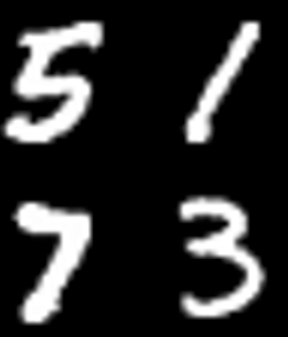
\includegraphics[width=0.25\linewidth]{mathworks_mnist_neuralnetFinal_v2}
		\caption{Sample numbers from MNIST \cite{mnistMATLAB2}.}
		\label{fig:mathworksmnistneuralnetfinal}
	\end{figure}
	
	\subsection{Artificial neural network}
	An artificial neural network (referred to as a neural network in this paper) is a computation system that mimics the biological neural networks found in animal brains. A neural network is not an algorithm, but a general framework to solve problems. Artificial neural networks are based of layers of interconnected neurons that transmit signals to each other. Neural networks may be trained for tasks, such as the number recognition in this report. 
	
	The neural net implemented in this project had an input vector of $784\times1$ and an output vector of $10\times1$. Different configurations were tried, with one hidden layer of $250\times1$ producing the best results. A visualization of an example neural net is seen in figure \ref{fig:nndiagram}.
	\begin{figure}
		\centering
		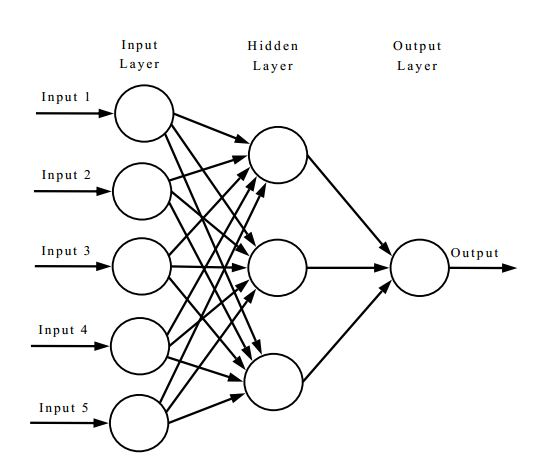
\includegraphics[width=0.6\linewidth]{nnDiagram}
		\caption{Visualization of a neural network with one hidden layer\cite{nnDiagramStack}. }
		\label{fig:nndiagram}
	\end{figure}
	
	
	\subsection{Neural Network Walkthrough}
	
	
	The training of a neural network involves four main steps:
	\begin{enumerate}\singlespacing
		\item Initialize weights and biases. 
		\item Forward propagation
		\item Compute the loss
		\item Backward propagation
	\end{enumerate}%\doublespacing



	\subsubsection{Parameter Initialization}
	The first step in training a neural net is to initialized the bias vectors and weight  matrices. They are initialized with random numbers between 0 and 1, then multiplied by a small scalar around the order of $10^{-2}$ so that the units are not on the region where the derivative of the activation function are close to zero. The initial parameters should be different values (to keep the gradients from being the same).
	
	There are various forms of initialization such as Xavier initialization or He-et-al Initialization, but a discussion on methods of initialization outside the scope of this paper. In this paper we will stick with random parameter initialization. 
	
	

	\subsubsection{Forward Propagation}
	The next step is the forward propagation. The network takes the inputs from a previous layer, computes their transformation, and applies an activation function. Mathematically the forward propagation at level ``i" is represented by equation~\ref{eqn:forProp}.\par  
	\begin{equation}
	\begin{aligned}
	z_i = A_{i-1}* W_{i}+b\\
	A_i=\phi(z_i)
	\end{aligned}
	\label{eqn:forProp}
	\end{equation}
	Where z is the input vector, A is the layer, W is the weights going into the layer, b the bias, and $\phi$ the activation function. This process then repeats for the next layer until it reaches the end of the neural net.
	
	\subsubsection{Compute loss}
	The loss is simply the difference between the output and the actual value. In this neural net it is computed by equation \ref{eqn:loss}.
	\begin{equation}
	\text{loss}=A_{i=\text{end}}-y
	\label{eqn:loss}
	\end{equation}
	This loss is used to begin the next step: backward propagation.
	\subsubsection{Backward propagation}
	
	After going forward through the neural net in the forward propagation step and computing the loss the final step is backwards propagation. Backwards propagation is the updating of the weight parameters via the derivative of the error function with respect to the weights of the neural net. For the output layer this is seen in equation \ref{eqn:outputBack} and equation \ref{eqn:allOtherBack} for all other layers.
	\begin{equation}
	dW_{i=\text{end}}=\phi'(z_{i=\text{end}})*\left(A_{i=\text{end}}-y\right)
	\label{eqn:outputBack}
	\end{equation}
	\begin{equation}
	dW_i=\phi'(z_i)*\left(W_{\left(i+1\right)}^T*dW_{\left(i+1\right)}\right)
	\label{eqn:allOtherBack}
	\end{equation}
	Once these derivatives have been computed, the weights are updated by equation \ref{eqn:updateWeight}
	\begin{equation}
	W_i = W_i=\alpha*dW_{i}*A_{\left(i-1\right)}^T
	\label{eqn:updateWeight}
	\end{equation}
	Where for the first layer $z_{\left(i-1\right)}^T$ will be the input vector and for all the following layers it will be the vector from the previous layer. \par 
	At this point the neural net has completed a full run through. The next input vector is selected and the forward and backward propagation are run again. A visualization of forward and backward propagation is in figure \ref{fig:forwardbackwardprop}.
	
	\begin{figure}
		\centering
		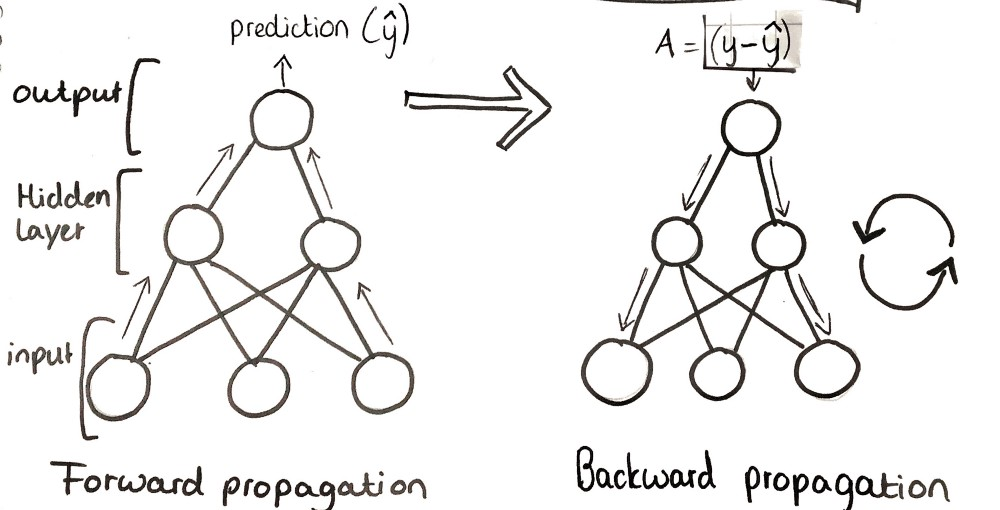
\includegraphics[width=0.7\linewidth]{forwardBackwardProp}
		\caption{A visualization of forward and backward propagation \cite{nnBlog}.}
		\label{fig:forwardbackwardprop}
	\end{figure}
	\subsection{Gradient Decent}
	Also known as steepest decent, gradient decent is a first order optimization algorithm. It is used to find the minimum of a function. Equation \ref{eqn:gdes} shows gradient decent implemented in a neural net. 
	
	\begin{equation}
	\Delta W(t) = - \alpha \frac{\partial E}{\partial W(t)}
	\label{eqn:gdes}
	\end{equation}
	Where $\alpha$ is the learning rate, and  $\partial E/\partial W(t)$ is the error derivative with respect to the weight. As these derivatives must be computed for each node the more nodes there are in a neural net the longer it will take to train. 
	\subsection{Activation Function}
	The activation function was previously mentioned as a function used to convert the input signal to the output signal. Activation functions introduce non-linear properties to the neural net's functions, allowing the neural net to represent complex functions \cite{nnBlog}. \par 
	The two most common activation functions used in neural nets for the gradient decent are sigmoid and hyperbolic tangent (Tanh). 
	The formula for Tanh is seen in equation \ref{eqn:tanH}, and the formula for it's derivative  is seen in equation \ref{eqn:dtanh} 
	\begin{equation}
	\phi_{\text{Tanh}}(z)=\frac{1-e^{-2z}}{1+e^{-2z}}
	\label{eqn:tanH}
	\end{equation}
	\begin{equation}
	\phi'_{\text{Tanh}}(z)=\frac{4}{\left(e^{-z}+e^{z}\right)^2}
	\label{eqn:dtanh}
	\end{equation}
	The formula for the sigmoid function is seen in equation \ref{eqn:sig}, the formula for it's derivative is seen in equation \ref{eqn:dsig}.
	
	\begin{equation}
	\phi_{\text{Sigmoid}}(z)=\frac{1}{1+e^{-z}}
	\label{eqn:sig}
	\end{equation}
	\begin{equation}
	\phi'_{\text{Sigmoid}}(z)=\frac{e^{-z}}{\left(e^{-z}+1\right)^2}
	\label{eqn:dsig}
	\end{equation}
	The sigmoid and Tanh function are visualized in figure \ref{fig:sigvstanh}.
	
	\begin{figure}
		\centering
		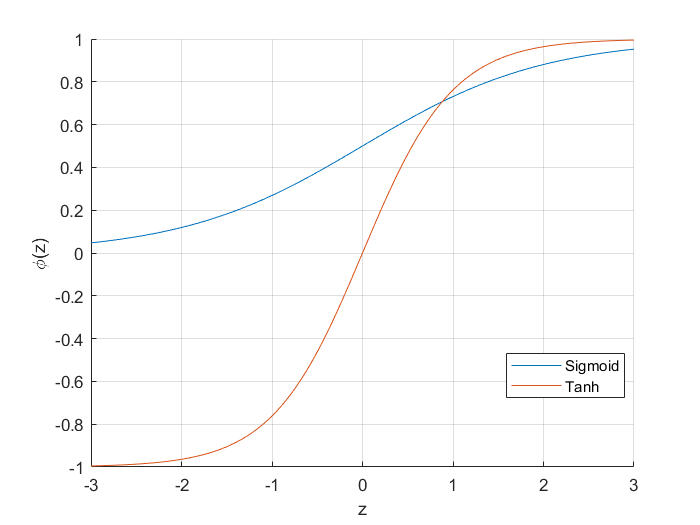
\includegraphics[width=0.4\linewidth]{sigVsTanh}
		\caption{Visualization of sigmoid and Tanh function}
		\label{fig:sigvstanh}
	\end{figure}

	Both functions have relatively simple mathematical formulas and are differentiable. In this paper the sigmoid function is used over the Tanh function as it had better results. Sigmoid and Tanh are not the only activation functions. Other functions that should be noted are the Rectified Linear Unit (ReLU) and the Leaky Rectified Linear Unit function. These functions have their own separate pros and cons, but a proper discussion of them is outside the scope of this paper. 
	
	\subsection{Pitfalls}
	The most important thing to steer clear of is over training. Over training occurs when the neural net trains too much to the training data. While it will have a high accuracy for the training data, it's performance for the test data will decay, as it has become too well attuned to the training data.  \par 
	
	The other problem is the time it takes to train. A three layer neural net can be trained to 97\% accuracy within 10 minutes, however it will not improve far beyond that. Larger nets will take longer to train, but will take far longer to train. 
	
	\begin{figure}
		\centering
		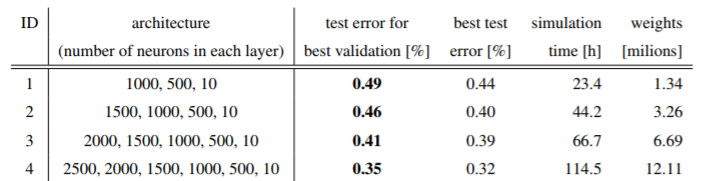
\includegraphics[width=0.7\linewidth]{nnRunTime}
		\caption{Run times for various neural network architectures\cite{deepBig}.}
		\label{fig:nnruntime}
	\end{figure}
	
	\section{Implementation}
	\subsection{Object Oriented Programming in MATLAB}
	This neural net had to be made without the use of any built in libraries \cite{Hicken18gradProjDes} and the code had to be modular \cite{Hicken18gradProjRubric}. To create code for neural network subject to these constraints the author decided to create their own neural net class in MATLAB. \par 
	
	
	The MATLAB class philipNeuralNet.m was written for this neural net project. It has the parameters learningRate, enableBias, actFunSwitch, and Level. The learningRate parameter is obviously the learning rate. The Level parameter has four parameters attached to it: W (weight), dW (weight derivative),  z (input), and A (the vector for the layer). By having this class we have avoided hard coding the propagation of the neural net and it is possible to test different neural net architectures on this code. \par 
	
	The MATLAB class also has an activation function and a derivative of the activation function. The actFunSwitch variable allows either the Sigmoid or the Tanh function to be selected. Additionally the enableBias variable allows for biases to be used or not used in the code's execution. \par 
	Finally it has a outputVector function that is simply an implementation of the neural net. It takes the input, runs it through the net, and returns the net's output. \par 
	
	
	
	\subsection{MATLAB Code}
	The MALAB code first initializes a neural net from given parameters. It obtains the MNIST data from a function\cite{usingMNIST}. It then uses the handleTrainNet function to train the net. This function implements batch training, using the forward and backward propagation functions. It then computes and displays the training error and the testing accuracy after a specified number of runs via the testAcc.m function. Once it has done this it plots the accuracy of the neural net via the plot accuracy function, generating the plots seen in the results section.
	 
	
	
	\section{Results}
	\subsection{Simple Neural Net}
	The best results were found for the simplest neural net examined; a one hidden layer with 250 nodes a learning rate of 0.1, and no biases. For this simple a test accuracy of 98\% was achieved. The first 1000 epochs of this net are visualized in figure \ref{fig:250_all}.
	\begin{figure}
		\centering
		\begin{subfigure}{.5\textwidth}
			\centering
			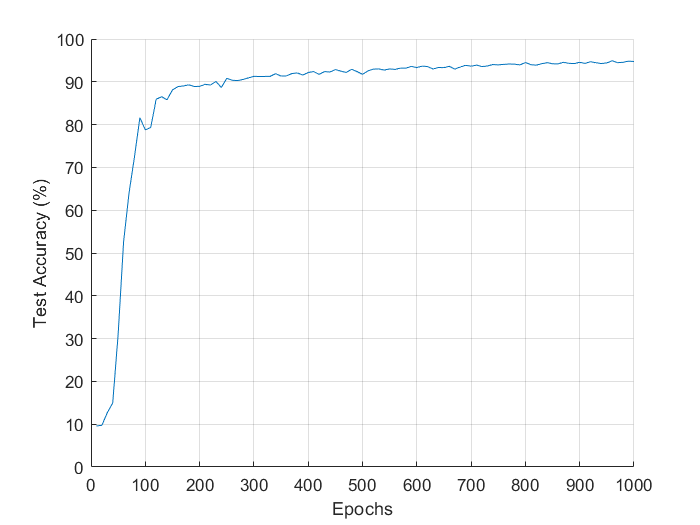
\includegraphics[width=\linewidth]{250_results}
			\caption{The results for the first 1000 epochs.}
			\label{fig:250results}
		\end{subfigure}%
		\begin{subfigure}{.5\textwidth}
			\centering
			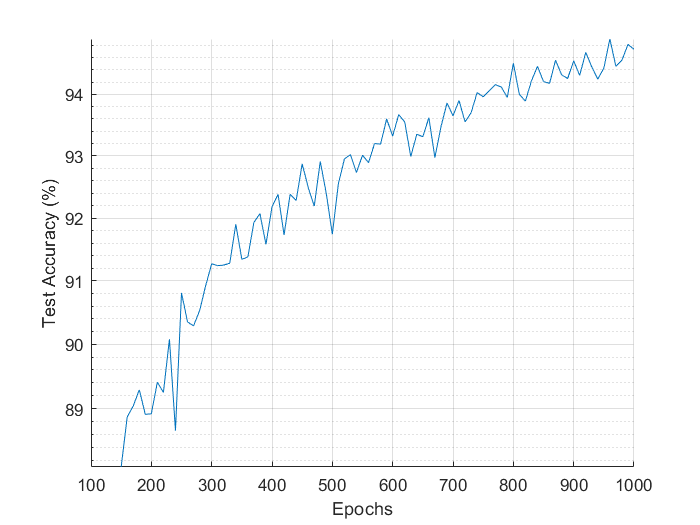
\includegraphics[width=\linewidth]{250_results_log}
			\caption{The results for the first epochs scaled logarithmically}
			\label{fig:250resultslog}
		\end{subfigure}
		\caption{The results from the simple network for the first 1000 epochs.}
		\label{fig:250_all}
	\end{figure}
	To get the 98.37\% accuracy it took approximately 12 hours of running the code and over three million neural net evaluations.
	
	\subsection{Comparison of different hidden layer sizes}
	
	From Shure \cite{matlabNNBeg}, the optimal size for the hidden layer in a three layer neural network for the MNIST is 250 nodes. Comparing the results for hidden layers show in figure \ref{fig:multiplelayers}, different sizes of hidden layer do not have a large effect on the accuracy of these results. However what is different is the time it takes to run each net. The more nodes in a net, the longer it takes for the net to train, as there are more operations to perform. Thus if a neural net with 250 nodes will have the same accuracy as a net with 800 nodes, the first net is preferable, as it will be trained faster.
	
	
	\begin{figure}
		\centering
		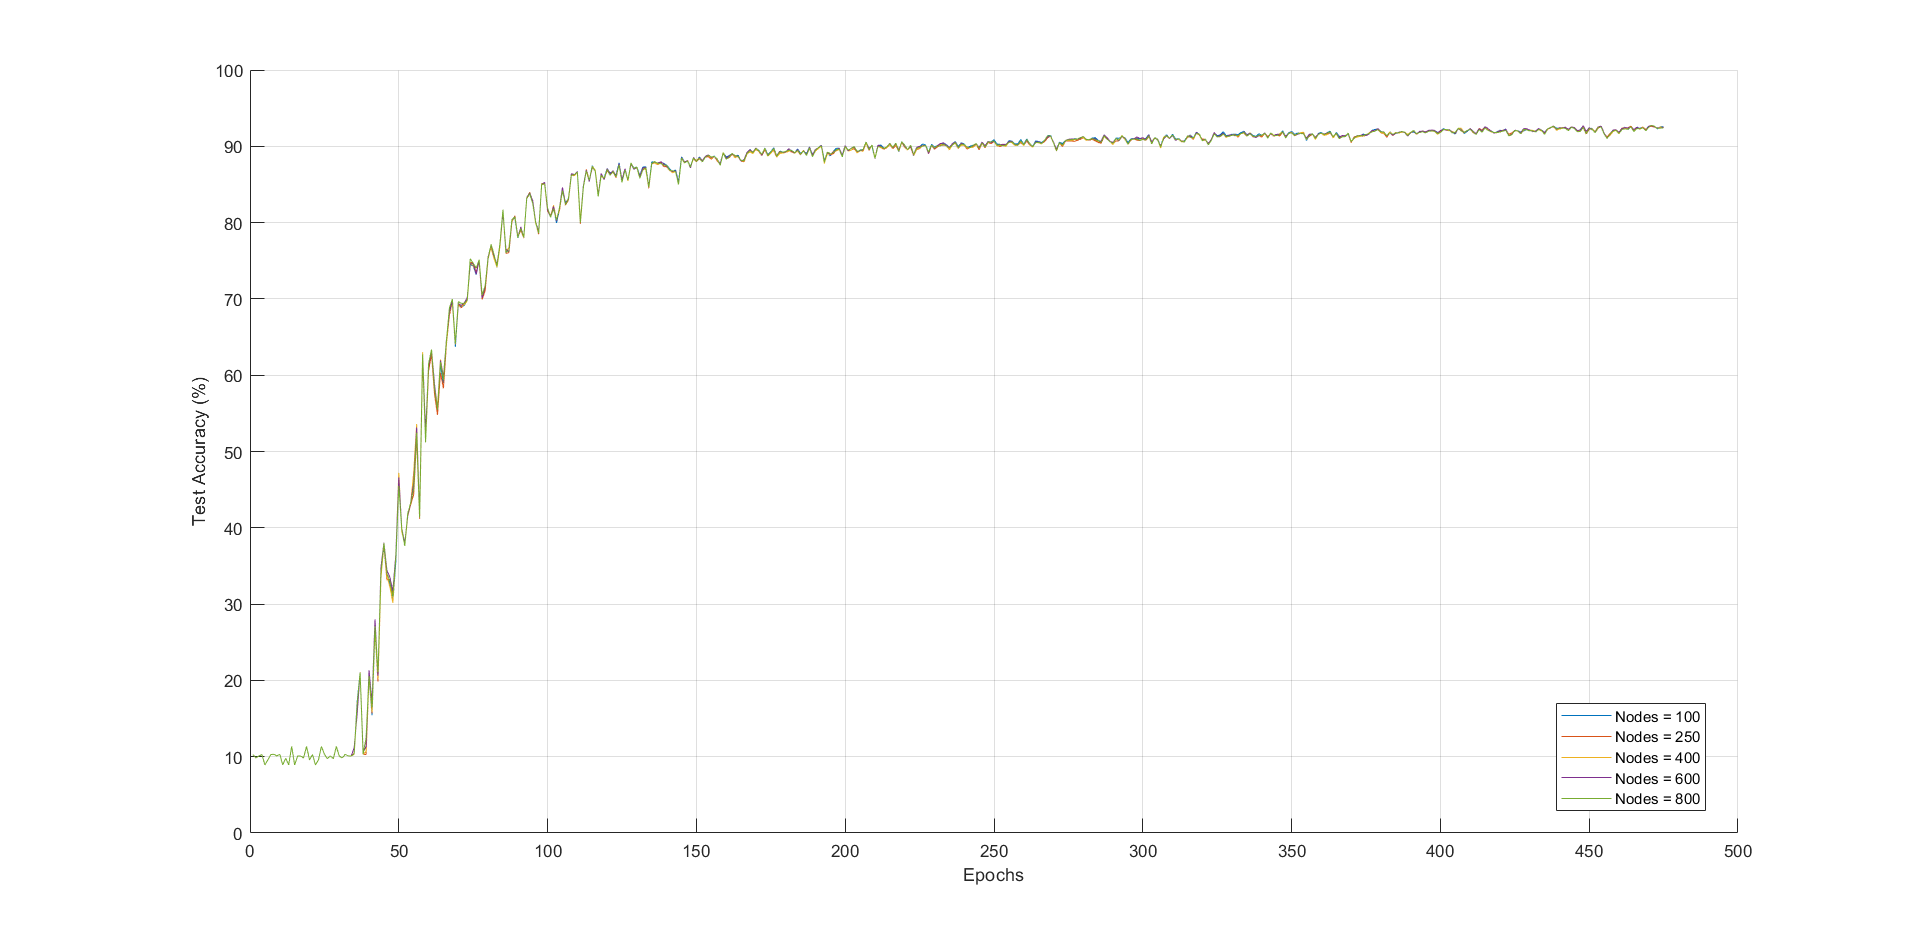
\includegraphics[width=0.7\linewidth]{multipleLayers}
		\caption{Net accuracy for different layer sizes.}
		\label{fig:multiplelayers}
	\end{figure}
	
	
	\subsection{Multiple hidden layers}
	The best accuracy occurred when both layers had a size of $250\times1$. For network with two hidden layers of 250 each the best test accuracy was 96.49\%. The accuracy from the first 2000 epochs is seen in figure \ref{fig:250_all_l2}. 
		\begin{figure}
		\centering
		\begin{subfigure}{.5\textwidth}
			\centering
			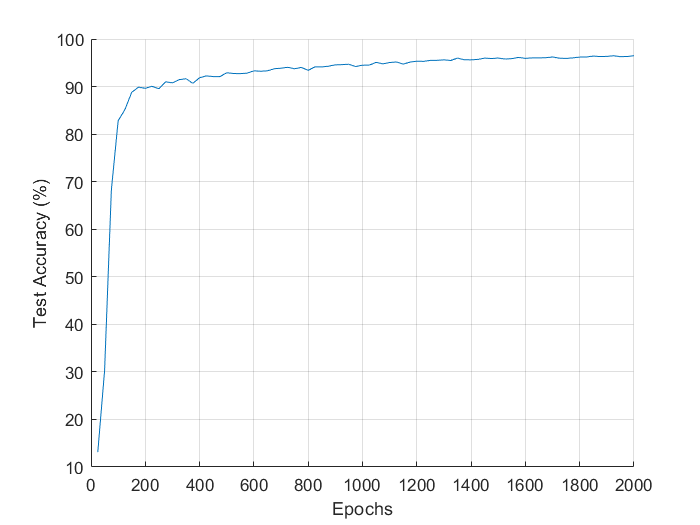
\includegraphics[width=\linewidth]{250_results_l2}
			\caption{The results for the first 2000 epochs.}
			\label{fig:250results_l2}
		\end{subfigure}%
		\begin{subfigure}{.5\textwidth}
			\centering
			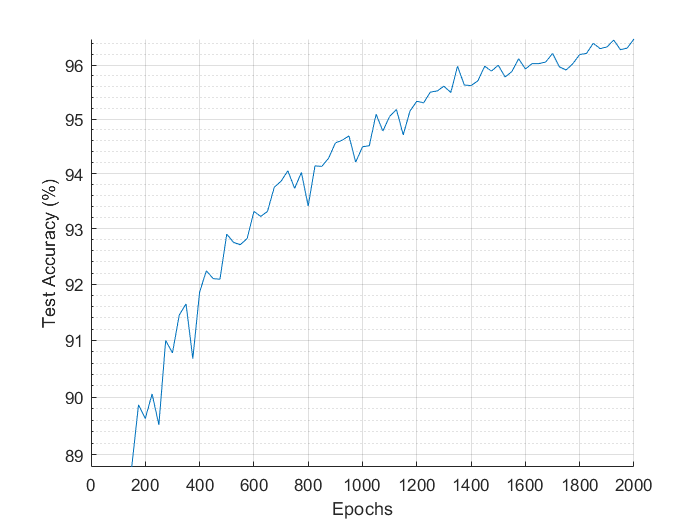
\includegraphics[width=\linewidth]{250_results_log_l2}
			\caption{The results for the first epochs scaled logarithmically}
			\label{fig:250resultslog_l2}
		\end{subfigure}
		\caption{The results from the two layer network for the first 2000 epochs.}
		\label{fig:250_all_l2}
	\end{figure}

	The accuracy of two hidden layers was not as good as the accuracy of one hidden layer. No other configurations achieved an accuracy as high as this one. 

	
	\section{Conclusion}
	
	The simple neural net achieved an accuracy of 98.37\%. This is on par with human recognition, and is about as accurate as a simple neural net can achieve. Higher accuracy rates are achieved via the use of constitutional neural networks, such as the  LeNet-5\cite{len5en}. Due to the long run time of large multi layered neural networks they were not studied, but could provide a more accurate identification with out convolution.\par 
	
	What is interesting is that the best results occurred with out biases and with one hidden layer. It was expected that adding more complexion to the neural net would increase the accuracy, however this was not the case. As neural nets are very much a trial and error process, it is possible that these more complex nets will achieve a better accuracy with more fiddling. 

			%--------------------------------------
		% References
		% -------------------------------------
		
		\bibliographystyle{unsrt}
		\bibliography{ref}

		
		%-----------------------------------------------------------
		% Appendix
		%-----------------------------------------------------------
		%\newpage
		\singlespacing
%		\section*{Appendix 1 -derivation of gibbs}
		\section*{Appendix 1 - MATLAB code}
		\addcontentsline{toc}{section}{Appendix}
		
		\lstset{language=Matlab,%
			%basicstyle=\color{red},
			breaklines=true,%
			morekeywords={matlab2tikz},
			keywordstyle=\color{blue},%
			morekeywords=[2]{1}, keywordstyle=[2]{\color{black}},
			identifierstyle=\color{black},%
			stringstyle=\color{mylilas},
			commentstyle=\color{mygreen},%
			showstringspaces=false,%without this there will be a symbol in the places where there is a space
			numbers=left,%
			numberstyle={\tiny \color{black}},% size of the numbers
			numbersep=9pt, % this defines how far the numbers are from the text
			emph=[1]{for,end,break},emphstyle=[1]\color{red}, %some words to emphasise
			%emph=[2]{word1,word2}, emphstyle=[2]{style},    
		}
	\subsection*{NN\_Master.m}
	%C:\Users\Philip\Documents\GitHub\DesignOpt\designOpNN\latexCode
	\lstinputlisting{C:/Users/Philip/Documents/GitHub/DesignOpt/designOpNN/latexCode/NN_Master.m}
	\subsection*{philipNeuralNet.m}
	\lstinputlisting{C:/Users/Philip/Documents/GitHub/DesignOpt/designOpNN/latexCode/philipNeuralNet.m}
	
	\subsection*{testAcc.m}
	\lstinputlisting{C:/Users/Philip/Documents/GitHub/DesignOpt/designOpNN/latexCode/testAcc.m}
	%\lstinputlisting{C:/Users/Philip/Documents/GitHub/Thesis/Master_TLE.m}
	%\lstinputlisting{C:/Users/Philip/Documents/GitHub/independent_study_fall_2018/Independat-Study-Fall-2018/Gibbs_Heck_master_loop_Latex.m}
	
	%\subsection{Code}
	%\subsection{Master\_TLE.m}
	%\lstinputlisting{C:/Users/Philip/Documents/GitHub/Thesis/Master_TLE.m}
	%\subsection{get\_SATCAT.m}
	%	\lstinputlisting{C:/Users/Philip/Documents/GitHub/Thesis/get_SATCAT.m}
	%	\subsection{get\_TLE\_from\_ID\_Manager.m}
	%\lstinputlisting{C:/Users/Philip/Documents/GitHub/Thesis/get_TLE_from_ID_Manager.m}
	
	%\subsection{get\_TLE\_from\_NorID.m}
	%\lstinputlisting{C:/Users/Philip/Documents/GitHub/Thesis/get_TLE_from_NorID.m}
	%\lstinputlisting{get_SATCAT.m}
	
	%Thanks for Paul McKee who started this template. It seems to have good matlab code viwing
		
	\end{document}
	
